\section{判定の基準を変えたとき}
\label{sec:sensitivity}

判定の基準は、どれもある程度は任意に決めた値である。値を 1 つずつ変えて、
標準の飛行で実施できる確率がどれだけ動くかを調べた（図~\ref{fig:sens}）。

\begin{description}
  \item[地上の風の上限] 最も効く。壱岐では上限を \SI{5}{\metre\per\second} から
    \SI{3}{\metre\per\second} に下げると \SI{29}{\percent} が \SI{15}{\percent} に半減し、
    \SI{7}{\metre\per\second} に上げると \SI{37}{\percent} になる。放球の技術と機材で
    許せる風速を決めることが、場所を選ぶことと同じくらい確率を左右する。
  \item[海岸から何 km までの海を認めるか] 0 km（瀬戸内海だけ）から \SI{10}{\kilo\metre} まで
    変えても、壱岐では \SIrange{28}{30}{\percent} とほとんど動かない。
    冬は落下点の多くが瀬戸内海か山地で、外海の海岸近くに落ちる日は少ないからである。
    平戸・大島と唐津・加唐島は \SIrange{30}{36}{\percent} と少し動く。
  \item[降水の上限] 9--12 時の降水を \SI{0.1}{\milli\metre} 未満にすると
    \SIrange{2}{4}{\percent} 下がり、\SI{2}{\milli\metre} 未満に緩めると同じくらい上がる。
  \item[瀬戸内海への着水] 認めない場合は、成功が平野と海岸近くの海だけになる。
    壱岐では実施できる確率が \SI{29}{\percent} から \SI{3}{\percent} 程度に、
    他の上位地点も \SIrange{3}{12}{\percent} に下がる（図~\ref{fig:breakdown} の成功の内訳）。
    瀬戸内海を使えないと、冬の西風で東へ \SI{250}{\kilo\metre} 流される先に、
    雪のない平野がまとまって広がる場所がほとんどない。
\end{description}

\begin{figure}[htbp]
\centering
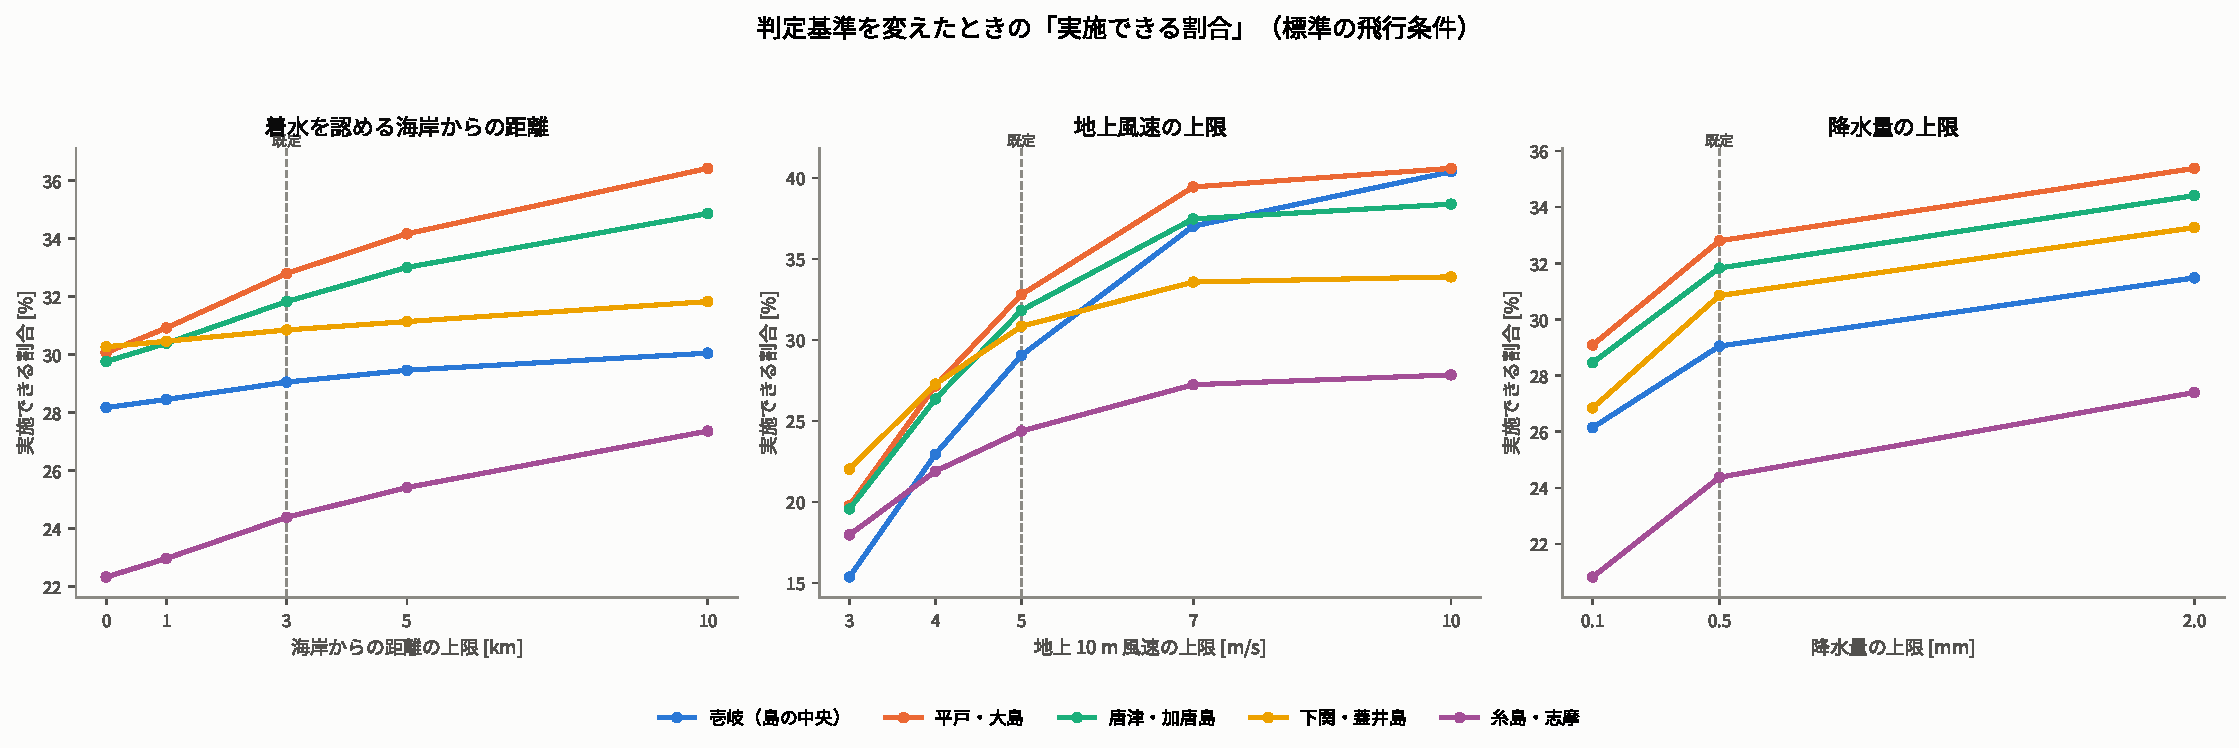
\includegraphics[width=\linewidth]{sensitivity.pdf}
\caption{判定の基準を変えたときの実施できる確率（標準の飛行）。
破線が本文で使った値（海岸から \SI{3}{\kilo\metre}、風 \SI{5}{\metre\per\second}、
降水 \SI{0.5}{\milli\metre}）。}
\label{fig:sens}
\end{figure}
